\subsection{Clustering evaluation}

\subsubsection{Hierarchical clustering parameters}

As explained in Section~\ref{sec:authors_clustering}, the hierarchical clustering decide clusters based on a bottom-up approach and have two main parameters, the stopping procedure and the linkage criterion.
The linkage criterion can be : single, complete, average linkage.
Oxquarry, Brunet, St-Jean A, St-Jean B and St-Jean copora are used for this experiment.
The goal is to understand how the linkage criterion behave in the following two best scenarios : when the right number of cluster is found ($r_{diff} = 0$) and the clustering with the best $B^3_{F_1}$.

The custom implementation of the hierarchical clustering is used, at each merging step, the intermediary clustering is evaluated using the two metrics.
The clustering resulting in the best $B^3_{F_1}$ is kept and the $r_{diff} = 0$.
This procedure is repeated for each linkage criteria and corpus.

The results for the two scenarios are presented in Table~\ref{tab:hierarchical_clustering}.
These results can be considered as the upper bound for the two metrics ($B^3_{F_1}$ and $r_{diff}$) for the clustering case using the retained rank list on these corpora.
Table~\ref{tab:hierarchical_clustering_rdiff_zero} represent the upper bound if the number of cluster is known for the hierarchical clustering with the retained rank lists and Table~\ref{tab:hierarchical_clustering_best_bcubed} the upper bound in case that the $B^3_{F_1}$ want to be maximized with the hierarchical clustering on the retained rank lists.
The best linkage criterion depends on the corpus, but in average, the best $B^3_{F_1}$ is achieved with the average linkage criterion, a relative increase of around 2.5\% compared to the other criteria.
Having a slightly greater number of cluster can produces in average a better $B^3_{F_1}$ score using the retained rank lists.

\begin{table}
  \centering
  \caption{Hierarchical clustering $B^3_{F_1}$/ $r_{diff}$ on every linkage criterion and corpus}
  \label{tab:hierarchical_clustering}

  \subcaption{Procedure stop at the right number of cluster ($r_{diff} = 0.00$)}
  \label{tab:hierarchical_clustering_rdiff_zero}
  \begin{tabular}{l c c c}
    \toprule
           & \multicolumn{3}{c}{Linkage criterion} \\
    Corpus    & Single    & Average   & Complete \\
    \midrule
    Oxquarry  & 0.81/0.00 & 0.93/0.00 & 0.81/0.00 \\
    Brunet    & 0.81/0.00 & 0.81/0.00 & 0.79/0.00 \\
    St-Jean A & 0.85/0.00 & 0.85/0.00 & 0.85/0.00 \\
    St-Jean B & 0.96/0.00 & 0.93/0.00 & 0.97/0.00 \\
    St-Jean   & 0.79/0.00 & 0.88/0.00 & 0.87/0.00 \\
    \midrule
    Mean      & 0.84/0.00 & 0.88/0.00 & 0.86/0.00 \\
    \bottomrule
  \end{tabular}

  \vspace{0.5cm}

  \subcaption{Best $B^3_{F_1}$ and its $r_{diff}$ across all hierarchical clustering stops}
  \label{tab:hierarchical_clustering_best_bcubed}
  \begin{tabular}{l c c c}
    \toprule
           & \multicolumn{3}{c}{Linkage criterion} \\
    Corpus    & Single     & Average   & Complete \\
    \midrule
    Oxquarry  & 0.89/ 0.04 & 0.96/0.02 & 0.87/0.04 \\
    Brunet    & 0.84/ 0.02 & 0.85/0.09 & 0.85/0.09 \\
    St-Jean A & 0.86/-0.01 & 0.88/0.03 & 0.88/0.04 \\
    St-Jean B & 0.98/ 0.02 & 0.98/0.02 & 0.97/0.00 \\
    St-Jean   & 0.87/ 0.09 & 0.89/0.01 & 0.90/0.01 \\
    \midrule
    Mean      & 0.89/0.03 & 0.91/0.02 & 0.89/0.02 \\
    \bottomrule
  \end{tabular}

\end{table}

\subsubsection{Unsupervised clustering evaluation}

For this experiment, the goal is to test the unsupervised hierarchical clustering cut method based on the maximization of the mean silhouette score on the literature corpora.
The right number of cluster is not known.
When applying the procedure, the number of clusters start at 2 and end at the number of documents minus 1.
The best clustering according to this method is the one that yield the greatest mean silhouette score, ref. Section~\ref{sec:unsupervised_clustering}.

The rank list used for this experiment is the one generated using Z-score fusion with retained text representation (9 for St-Jean and 7 for Brunet and Oxquarry), see Section~\ref{sec:annex_retained_text_representation} in annex.

The detailed $B^3_{F_1}$ and score on the unsupervised clustering is presented in Table~\ref{tab:unsupervised_clustering_0}.
An example of the best case and worse case are presented Figures~\ref{fig:unsupervised_clustering}.
The silhouette score is indicated as each step and compared to clustering evaluation metrics.

Since the rank list used for the clustering is not perfect (every true links at the top), there is no number of cluster with a BCubed $F_1$ score of 1.0.
The estimated number of cluster is on every dataset overestimated, since the average r-ratio difference is positive value ranging between $\left[0.16, 0.20\right]$ depending on the linkage criterion, which means that the mean neareast-cluster distance is greater than the mean intra-cluster distance even when dealing with the right number of clusters.
This can be due to the fact that the rank list used for the clustering is not perfect (AP $\neq 1$).

To mitigate this problem, an easy solution would be to use the labels produced by the clustering of a non-maximal value of the silhouette score on the left side of the maximal silhouette score.
In this study, we introduce a parameter called $\alpha$. Alpha represents a percentage of value to subtract to the maximal mean silhouette score to obtain the new target (instead of the maximal value).
The sign of the alpha indicate on the side of the maximal silhouette score the target should be.
With $\alpha = 0$, this corresponds to the maximal mean silhouette score.
With a negative $\alpha$ the left side is targeted and with a positive $\alpha$, the right side.
By using for example $\alpha = -0.3$, we aim to correct this overshoot.
Table~\ref{tab:unsupervised_clustering_03} show the results with this $\alpha$.
With this correction technique, the average $B^3_{F_1}$ can be increase by ~11\% across all the corpora.

\begin{table}
  \centering
  \caption{Unsupervised clustering evaluation on every linkage criterion and corpus}
  \label{tab:unsupervised_clustering}

  \caption{$\alpha = 0$}
  \label{tab:unsupervised_clustering_0}
  \begin{tabular}{l c c c}
    \toprule
           & \multicolumn{3}{c}{Linkage criterion} \\
    Corpus    & Single     & Average   & Complete \\
    \midrule
    Oxquarry  & 0.80/0.10 & 0.80/0.10 & 0.80/0.10 \\
    Brunet    & 0.67/0.32 & 0.72/0.20 & 0.70/0.25 \\
    St-Jean A & 0.57/0.30 & 0.57/0.29 & 0.60/0.25 \\
    St-Jean B & 0.89/0.08 & 0.91/0.05 & 0.91/0.05 \\
    St-Jean   & 0.70/0.21 & 0.74/0.15 & 0.71/0.17 \\
    \midrule
    Mean      & 0.72/0.20 & 0.75/0.16 & 0.74/0.16 \\
    \bottomrule
  \end{tabular}

  \subcaption{$\alpha = -0.3$}
  \label{tab:unsupervised_clustering_03}
  \begin{tabular}{l c c c}
    \toprule
           & \multicolumn{3}{c}{Linkage criterion} \\
    Corpus    & Single     & Average   & Complete \\
    \midrule
    Oxquarry  & 0.81/0.00 & 0.93/ 0.00 & 0.84/ 0.02 \\
    Brunet    & 0.81/0.00 & 0.79/ 0.02 & 0.79/ 0.05 \\
    St-Jean A & 0.81/0.07 & 0.82/ 0.07 & 0.81/ 0.06 \\
    St-Jean B & 0.83/0.05 & 0.82/-0.06 & 0.85/-0.06 \\
    St-Jean   & 0.81/0.01 & 0.86/-0.03 & 0.84/-0.03 \\
    \midrule
    Mean      & 0.81/0.01 & 0.85/0.00 & 0.83/0.01 \\
    \bottomrule
  \end{tabular}
\end{table}

\begin{figure}
  \caption{Unsupervised clustering example the worse (St-Jean A) and best (St-Jean B) clustering with the average linkage criterion}
  \label{fig:unsupervised_clustering}

  \subcaption{St-Jean A}
  \label{fig:unsupervised_clustering_st_jean_A_average}
  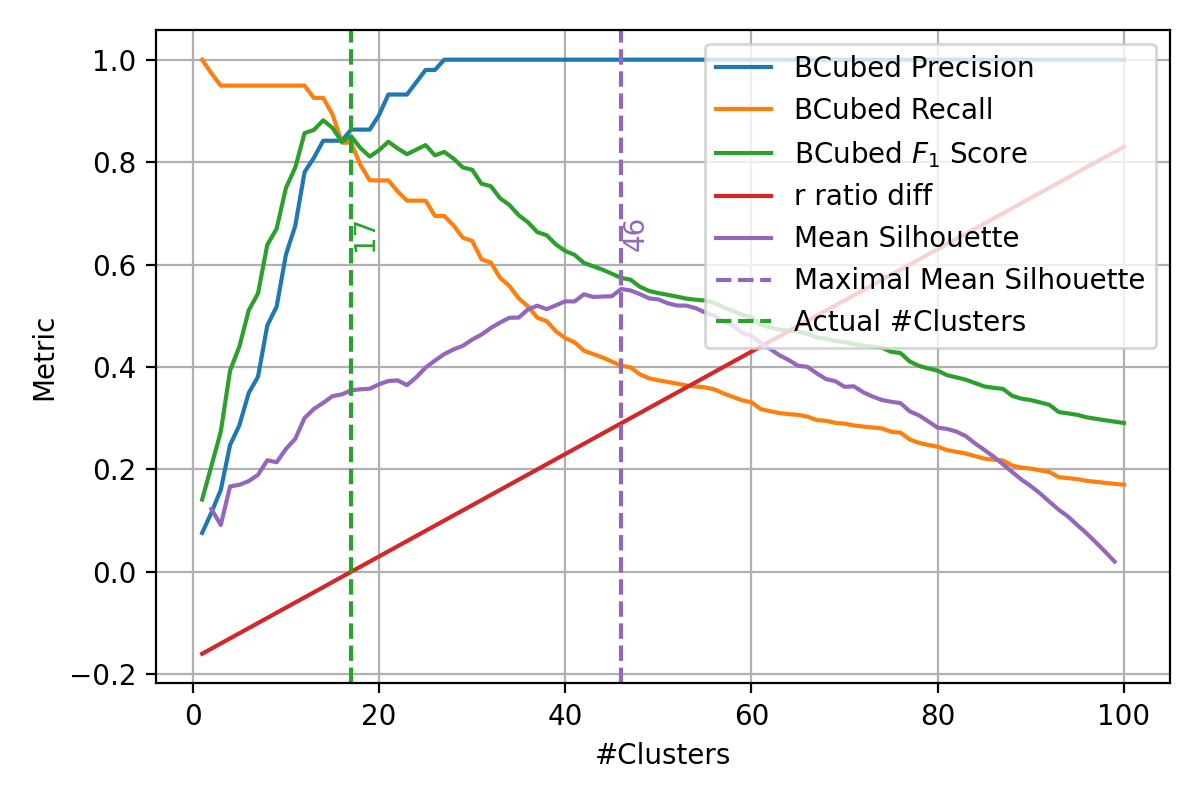
\includegraphics[width=\linewidth]{img/unsupervised_clustering_st_jean_A_average.png}

  \vspace{0.5cm}

  \subcaption{St-Jean B}
  \label{fig:unsupervised_clustering_st_jean_B_average}
  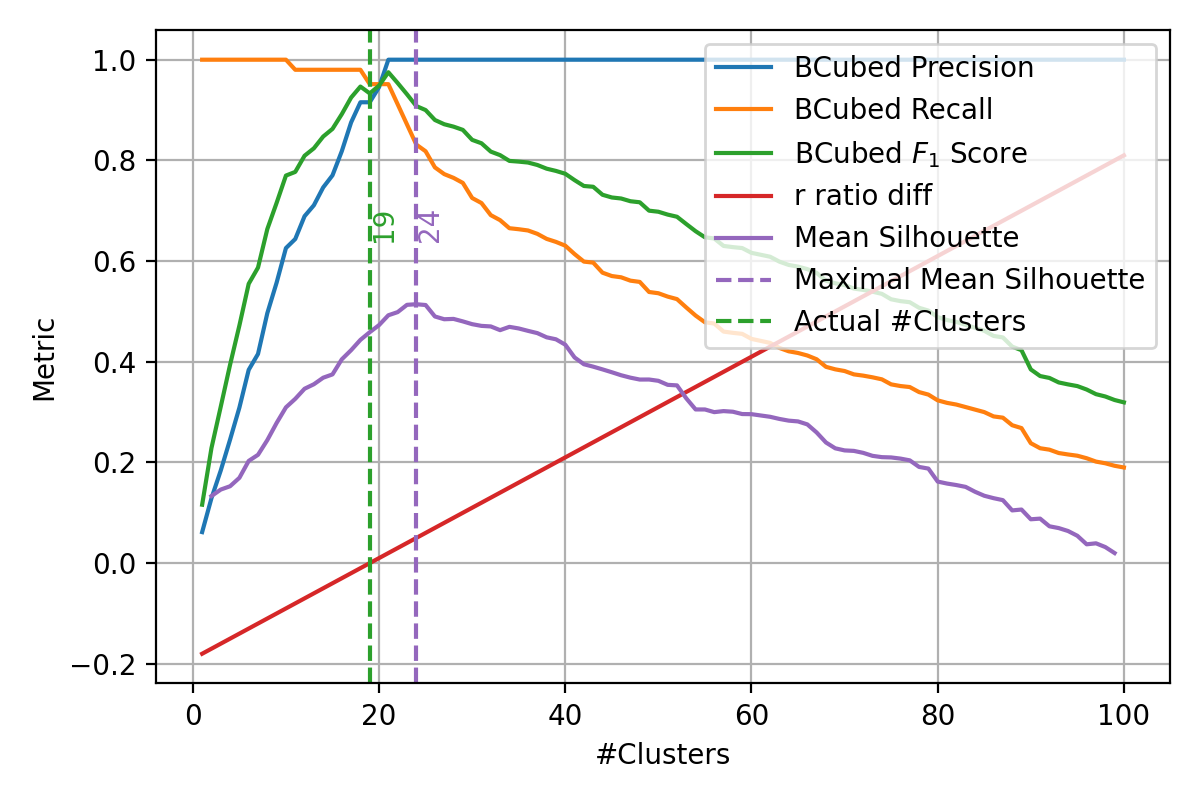
\includegraphics[width=\linewidth]{img/unsupervised_clustering_st_jean_B_average.png}
\end{figure}


\subsubsection{Semi-supervised clustering evaluation}

To evaluate the semi-supervised clustering approach, every corpus were used.
First a rank list for each corpus is computed using a z-score fusion using the retained rank list, see Section~\ref{sec:annex_retained_text_representation} in annex.
For each rank list, the distance threshold is computed, using the two beta approach, this correspond to the training phase.
Then for every distance threshold and rank list pair, the clustering is evaluated using the $B^3$ family and the $r_{diff}$.

The distance thresholds found for the z-score fusion rank lists for each corpus are in Table~\ref{tab:semi_supervised_clustering_thresholds}
The complete evaluation using Oxquarry, Brunet, St-Jean A and B, is presented in Table~\ref{tab:semi_supervised_clustering_train_test}.
The average values obtained for each metrics is presented in Table~\ref{tab:semi_supervised_clustering_average}.

The following conclusions can be drawn with these results:
\begin{itemize}
  \item
  A rather wide range of distance threshold is found depending on the corpus. They are in the interval $\left[-0.42, -0.96\right]$ which correspond to 14\% of the interval containing every z-scores for these datasets ($\left[-4.79, 2.63\right]$).
  \item
  The average r-ratio is positive, which indicate that this method tends to overestimate the number of clusters, but is really close to find the right number of clusters.
  \item
  The better the average precision of the rank list used, the better the $B^3_{F_1}$ score seem to be, when using this method, with the exception of the Oxquarry corpus which have better average precision then Brunet but a lower $B^3_{F_1}$ score in average when testing with these corpora.
  \item
  The distance threshold use only have a slight impact when comparing the average $B^3_{F_1}$ score across the corpus.
  The St-Jean A corpus give the best $B^3_{F_1}$ and regarding the number of clusters Oxquarry seem to be the best corpus for the training.
\end{itemize}

The semi-supervised cut method tends to produce better results in average than the unsupervised proposed method.
An increase of +8\% in $B^3_{F_1}$ can be obtained when using the supervised clustering model proposed over the unsupervised tweaked clustering model (IPS stop procedure at 0.1) and +15\% over the IPS stop procedure at 0.

\begin{table}
  \centering
  \caption{Distance threshold found with the two beta distribution on every corpora when using the z-score fusion of the retained rank lists}
  \label{tab:semi_supervised_clustering_thresholds}

  \begin{tabular}{l r}
    \toprule
    Corpus & Threshold \\
    \midrule
    Oxquarry & -0.42 \\
    Brunet & -0.62 \\
    St-Jean A & -0.76 \\
    St-Jean B & -0.96 \\
    \bottomrule
  \end{tabular}
\end{table}

\begin{table*}
  \centering
  \caption{Semi-supervised clustering evaluation}
  \label{tab:semi_supervised_clustering}

  \subcaption{Every possible distance threshold (DT) and retained z-score rank list pairs. Metrics in order : $B^{3}_{F_1}$ / $B^{3}_{precision}$ / $B^{3}_{recall}$ / $r_{diff}$}
  \label{tab:semi_supervised_clustering_train_test}
  \begin{tabular}{l l| c c c c}
    \toprule
    \multicolumn{2}{c}{\multirow{2}{*}{}} & \multicolumn{4}{c}{Testing} \\
    \multicolumn{2}{c}{} & Oxquarry & Brunet & St-Jean A & St-Jean B \\
    \midrule
    \parbox[t]{2mm}{\multirow{4}{*}{\rotatebox[origin=c]{90}{DT}}}
    & Oxquarry
    & 0.82/1.00/0.70/0.08
    & 0.81/0.85/0.77/0.07
    & 0.86/0.84/0.87/-0.02
    & 0.91/0.86/0.98/-0.03
    \\
    & Brunet
    & 0.82/1.00/0.70/0.08
    & 0.81/0.85/0.77/0.07
    & 0.87/0.86/0.87/-0.01
    & 0.92/0.88/0.98/-0.02
    \\
    & St-Jean A
    & 0.82/1.00/0.70/0.08
    & 0.85/0.94/0.77/0.09
    & 0.87/0.86/0.87/-0.01
    & 0.97/0.97/0.98/0.00
    \\
    & St-Jean B
    & 0.80/1.00/0.67/0.10
    & 0.84/1.00/0.73/0.14
    & 0.84/0.93/0.77/0.04
    & 0.90/0.97/0.83/0.04
    \\
    \bottomrule
  \end{tabular}

  \vspace{0.5cm}

  \subcaption{Metrics averages}
  \label{tab:semi_supervised_clustering_average}
  \begin{tabular}{l c c c c}
    \toprule
    & $B^{3}_{F_1}$
    & $B^{3}_{precision}$
    & $B^{3}_{recall}$
    & $r_{diff}$ \\
    \midrule
    Testing on Oxquarry               & 0.82 & 1.00 & 0.69 &  0.08 \\
    Testing on Brunet                 & 0.83 & 0.91 & 0.76 &  0.09 \\
    Testing on St-Jean A              & 0.86 & 0.88 & 0.85 &  0.00 \\
    Testing on St-Jean B              & 0.93 & 0.92 & 0.94 & -0.00 \\
    Distance threshold from Oxquarry  & 0.85 & 0.89 & 0.83 & 0.02 \\
    Distance threshold from Brunet    & 0.86 & 0.90 & 0.83 & 0.03 \\
    Distance threshold from St-Jean A & 0.88 & 0.94 & 0.83 & 0.04 \\
    Distance threshold from St-Jean B & 0.85 & 0.98 & 0.75 & 0.08 \\
    \textbf{Global average} & \textbf{0.86} & \textbf{0.93} & \textbf{0.81} & \textbf{0.04} \\
    \bottomrule
  \end{tabular}
\end{table*}

\subsubsection{Supervised clustering evaluation}

To evaluate the supervised clustering approach, every dataset were used.
First a rank list for each dataset is computed using a z-score fusion using the retained rank list, see Section~\ref{sec:annex_retained_text_representation} in annex.
Then every pair of rank list is used to create a training/testing evaluation.
In other words, a model to create cuts is trained on every dataset and tested on all the datasets.

The model does not depend on the rank list size since only relative magnitudes are used.
The BCubed $F_1$ metrics and the r ratio difference are computed during this experiment and are in presented in Table~\ref{tab:supervised_clustering_train_test}, for every pairs of dataset.
The average values obtained for each metrics is presented in Table~\ref{tab:supervised_clustering_average}.

Two conclusion can be drawn with these results:
\begin{itemize}
  \item
  When testing the cut model, having a rank list of good quality tends to produce better clustering, no matter the quality of the rank list used for the training.
  When testing the clustering model on St-Jean B (the corpus with the best rank list obtained, 0.96 AP), it obtains in average the best $B^3_{F_1}$ 0.93 for any training model.
  The least performing rank list also have the least accurate results during the clustering task, Brunet with 0.76 AP have an average clustering $B^3_{F_1}$ of 0.80.
  \item
  Using the best rank list for training the cut model does not always give the best results.
  An example to illustrate this observation, the St-Jean B dataset have the best rank list with an average precision of 0.96, but the best rank list for training the clustering model is Oxquarry with an average $r_{diff}$ of 0.02 and an average $B^3_{F_1}$ of 0.87.
  In the other hand, St-Jean B have an average $r_{diff}$ of 0.09 and an average $B^3_{F_1}$ of 0.83.
  The Oxquarry rank list seem to be the best dataset to train the model to perform the cut and Brunet the least effective.
\end{itemize}

The conclusion to the two previous points is that having a good rank list is more important for testing than training.
No clear rank lists property was found which makes some of them better to train the model.
The supervised cut method tends to produce better results in average than the unsupervised proposed method.
An increase of +8\% in $B^3_{F_1}$ can be obtained when using the supervised clustering model proposed over the unsupervised tweaked clustering model (IPS stop procedure at 0.1) and +14\% over the IPS stop procedure at 0.

\begin{table*}
  \centering
  \caption{Supervised clustering evaluation}
  \label{tab:supervised_clustering}

  \subcaption{Every possible threshold and dataset pairs. Metrics in order : $B^{3}_{F_1}$ / $B^{3}_{precision}$ / $B^{3}_{recall}$ / $r_{diff}$}
  \label{tab:supervised_clustering_train_test}
  \begin{tabular}{l l| c c c c}
    \toprule
    \multicolumn{2}{c}{\multirow{2}{*}{}} & \multicolumn{4}{c}{Testing} \\
    \multicolumn{2}{c}{} & Oxquarry & Brunet & St-Jean A & St-Jean B \\
    \midrule
    \parbox[t]{2mm}{\multirow{4}{*}{\rotatebox[origin=c]{90}{Training}}}
    & Oxquarry
    & 0.82/1.00/0.70/0.08
    & 0.86/0.91/0.82/0.07
    & 0.88/0.84/0.93/-0.03
    & 0.92/0.88/0.98/-0.02
    \\
    & Brunet
    & 0.80/1.00/0.67/0.10
    & 0.75/0.94/0.62/0.18
    & 0.81/0.98/0.69/0.09
    & 0.91/1.00/0.83/0.05
    \\
    & St-Jean A
    & 0.80/1.00/0.67/0.10
    & 0.82/0.94/0.73/0.11
    & 0.87/0.93/0.81/0.03
    & 0.97/1.00/0.94/0.02
    \\
    & St-Jean B
    & 0.80/1.00/0.67/0.10
    & 0.76/0.94/0.64/0.16
    & 0.82/0.96/0.72/0.07
    & 0.93/1.00/0.87/0.04
    \\
    \bottomrule
  \end{tabular}

  \vspace{0.5cm}

  \subcaption{Metrics averages}
  \label{tab:supervised_clustering_average}
  \begin{tabular}{l c c c c}
    \toprule
    & $B^{3}_{F_1}$
    & $B^{3}_{precision}$
    & $B^{3}_{recall}$
    & $r_{diff}$ \\
    \midrule
    Testing on Oxquarry     & 0.81 & 1.00 & 0.68 & 0.09 \\
    Testing on Brunet       & 0.80 & 0.93 & 0.70 & 0.13 \\
    Testing on St-Jean A    & 0.85 & 0.93 & 0.79 & 0.04 \\
    Testing on St-Jean B    & 0.93 & 0.97 & 0.91 & 0.02 \\
    Training on Oxquarry    & 0.87 & 0.91 & 0.86 & 0.02 \\
    Training on Brunet      & 0.82 & 0.98 & 0.71 & 0.10 \\
    Training on St-Jean A   & 0.86 & 0.97 & 0.79 & 0.06 \\
    Training on St-Jean B   & 0.83 & 0.97 & 0.73 & 0.09 \\
    \textbf{Global average} & \textbf{0.85} & \textbf{0.96} & \textbf{0.77} & \textbf{0.07} \\
    \bottomrule
  \end{tabular}
\end{table*}
